%
% GradingRubric.tex
% This page will be the 2nd page of your report and will be used for grading the homework/assignment.
\section*{Grading Rubric - Information to Students}

Grading rubric that will broadly apply to assessing performance. That is, assessment exercises that are associated with a predominantly qualitative rather than quantitative character. If, for a particular exercise, there is substantial deviation from the scheme outlined below, I will let you know! Note: Be aware that if your “Quality of Presentation” is poor, it could impact scores assigned for the other two categories! (DO NOT EDIT THIS PAGE)
%\hspace*{-1.5in}
\begin{figure}[ht!]
    \centering
    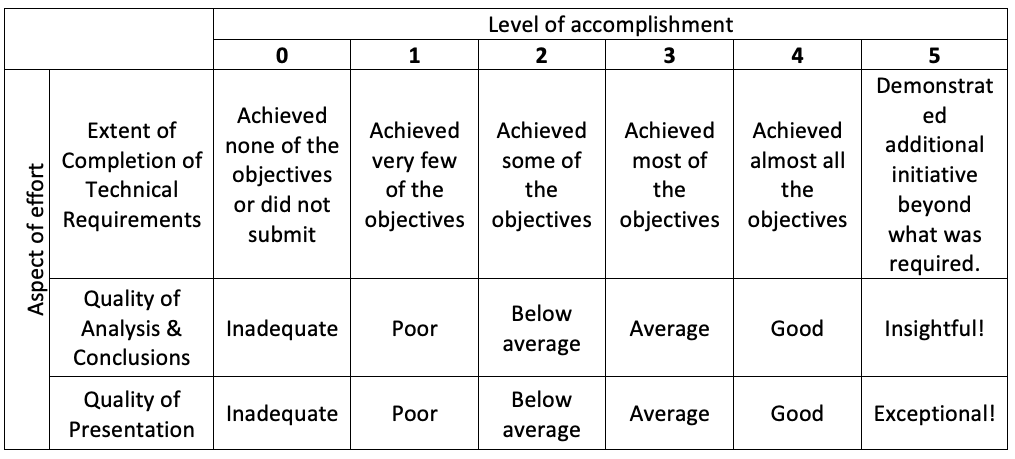
\includegraphics[scale=0.450]{LevelOfAccomplishments.png}
    \caption{Level of accomplishments}
    \label{fig:Level of accomplishments}
\end{figure}
\begin{table}[h]
    \centering
    \begin{tabular}{|c|c|}
    \hline
        Level &  Score \\
        \hline
        \hline
        5 &  12 (bonus!) \\
        \hline
        4: (`A`) &  10 \\
        \hline
        3: (`B`) &  8 \\
        \hline
        2: (`C`) &  6 \\
        \hline
        1: (`D`) &  4 \\
        \hline
        0: (`F`) &  0-2 \\
        \hline
    \end{tabular}
    \caption{Mapping of “Level” to “Score”}
    \label{tab:Mapping}
\end{table}
\begin{itemize}
    \item \textbf{Student's Level/Score (To be entered by Professor/GTA):}
\end{itemize}


